% QUESTAO
A \'area do ret\^angulo abaixo \'e de $24$\,m$^2$. Assim, o valor de $x$ \'e:

\parbox{0.35\linewidth}{

% ALTERNATIVAS
$4$\,m
$3$\,m
$5$\,m
$6$\,m
$7$\,m

}\parbox{0.64\linewidth}{
\begin{center}
\vspace{-6mm}
\begin{tikzpicture}[ rotate=0 ]
\retangulo{$x+2$}{6}{$x$}{4};
\end{tikzpicture}
\vspace{-9mm}
\end{center}
}


